% =========================================================================
%  AgentPwn: A Security Testing Framework for Agentic AI Systems
%  USENIX Security-style paper
% =========================================================================
\documentclass[letterpaper,twocolumn,10pt]{article}

% ---------- Packages ----------
\usepackage[utf8]{inputenc}
\usepackage[T1]{fontenc}
\usepackage{times}
\usepackage{microtype}
\usepackage{graphicx}
\usepackage{booktabs}
\usepackage{multirow}
\usepackage{array}
\usepackage{tabularx}
\usepackage{xcolor}
\usepackage{listings}
\usepackage{amsmath,amssymb}
\usepackage{enumitem}
\usepackage{balance}
\usepackage{url}
\usepackage[breaklinks]{hyperref}
\usepackage{fancyhdr}
\usepackage{float}
\usepackage{caption}
\usepackage{subcaption}
\usepackage{tikz}
\usetikzlibrary{shapes,arrows.meta,positioning,fit,calc,backgrounds}
\usepackage[ruled,vlined,linesnumbered]{algorithm2e}
\usepackage{natbib}

% ---------- Page geometry (USENIX-like) ----------
\usepackage[top=1in,bottom=1in,left=0.75in,right=0.75in]{geometry}
\setlength{\columnsep}{0.25in}

% ---------- Hyperref config ----------
\hypersetup{
  colorlinks=true,
  linkcolor=blue!60!black,
  citecolor=blue!60!black,
  urlcolor=blue!60!black,
}

% ---------- Code listing style ----------
\definecolor{codebg}{HTML}{F5F5F5}
\definecolor{codeframe}{HTML}{CCCCCC}
\definecolor{codekw}{HTML}{0000AA}
\definecolor{codecomment}{HTML}{008000}
\definecolor{codestring}{HTML}{AA0000}

\lstset{
  language=Python,
  basicstyle=\small\ttfamily,
  keywordstyle=\color{codekw}\bfseries,
  commentstyle=\color{codecomment}\itshape,
  stringstyle=\color{codestring},
  backgroundcolor=\color{codebg},
  frame=single,
  rulecolor=\color{codeframe},
  breaklines=true,
  breakatwhitespace=false,
  showstringspaces=false,
  tabsize=4,
  xleftmargin=1em,
  framexleftmargin=0.5em,
  numbers=left,
  numberstyle=\tiny\color{gray},
  numbersep=5pt,
  captionpos=b,
  aboveskip=0.8em,
  belowskip=0.5em,
}

\lstdefinelanguage{yaml}{
  keywords={true,false,null,yes,no},
  sensitive=false,
  comment=[l]{\#},
  morestring=[b]',
  morestring=[b]",
}

% ---------- Severity color badges ----------
\newcommand{\critical}{\textcolor{red!80!black}{\textbf{CRITICAL}}}
\newcommand{\high}{\textcolor{orange!80!black}{\textbf{HIGH}}}
\newcommand{\medium}{\textcolor{yellow!60!black}{\textbf{MEDIUM}}}
\newcommand{\low}{\textcolor{blue!70!black}{\textbf{LOW}}}
\newcommand{\info}{\textcolor{gray}{\textbf{INFO}}}

% ---------- Custom commands ----------
\newcommand{\apwn}{\textsc{AgentPwn}}
\newcommand{\ie}{\textit{i.e.}}
\newcommand{\eg}{\textit{e.g.}}
\newcommand{\etal}{\textit{et al.}}
\newcommand{\code}[1]{\texttt{#1}}
\newcommand{\Cref}[1]{Section~\ref{#1}}
\newcommand{\Tref}[1]{Table~\ref{#1}}
\newcommand{\Fref}[1]{Figure~\ref{#1}}
\newcommand{\Aref}[1]{Algorithm~\ref{#1}}

% ---------- Header ----------
\pagestyle{fancy}
\fancyhf{}
\fancyhead[L]{\small\textit{AgentPwn: A Security Testing Framework for Agentic AI Systems}}
\fancyhead[R]{\small\thepage}
\renewcommand{\headrulewidth}{0.4pt}

% ===== BEGIN DOCUMENT =====

\begin{document}

% ---------- Title Block ----------
\title{\Large\textbf{AgentPwn: A Modular Security Testing Framework\\for Agentic AI Systems}}

\author{
  \textbf{Wyatt Matson}\\
  Matson Capital Group LLC\\
  \texttt{wyatt@matsoncapitalgroup.com}
}

\date{}
\maketitle
\thispagestyle{fancy}

% ===================================================================
%  ABSTRACT
% ===================================================================

\begin{abstract}
The rapid adoption of agentic AI systems---autonomous LLM-based agents with tool access, external data retrieval, and inter-agent communication---has created novel attack surfaces that existing security testing tools are not designed to evaluate.
We present \apwn{}, the first open-source security testing framework purpose-built for agentic AI systems.
\apwn{} introduces a formal vulnerability taxonomy of five attack categories---prompt injection, tool manipulation, privilege escalation, multi-agent attacks, and MCP protocol attacks---implemented across 16 attack modules comprising 176 adversarial payloads.
The framework provides a modular, plugin-based architecture with auto-discovered attack modules, six framework-agnostic target connectors (OpenAI, Anthropic, LangChain, CrewAI, MCP, and custom HTTP), and multi-format report generation with weighted risk scoring.
We evaluate \apwn{} against simulated agent configurations across four vulnerability levels and demonstrate its ability to systematically identify and classify vulnerabilities that span trust boundaries unique to agentic systems.
Our evaluation reveals that tool output injection and MCP-based attacks represent the most critical threat vectors, with agents at medium vulnerability levels succumbing to over 50\% of prompt injection payloads.
\apwn{} maps all findings to established standards including MITRE ATLAS, OWASP LLM Top~10 (2025), and 14~CWE identifiers, enabling integration into existing security workflows.
The framework and all attack modules are released under the Apache~2.0 license.
\end{abstract}

% ===================================================================
%  1. INTRODUCTION
% ===================================================================

\section{Introduction}
\label{sec:intro}

Large language models (LLMs) have rapidly evolved from conversational assistants into autonomous agents capable of planning, reasoning, and executing actions in the real world~\citep{wang2024survey, yao2023react, schick2023toolformer}.
These \textit{agentic AI systems} operate by receiving instructions, deciding which tools to invoke (APIs, databases, code interpreters), observing results, and iterating until a goal is met.
The deployment of such systems in production environments---from customer service bots with CRM access to code generation agents with file system permissions---has introduced security risks that are fundamentally different from those of traditional software.

Unlike conventional applications, where inputs and outputs traverse well-understood trust boundaries, agentic AI systems blur the distinction between \textit{instructions} (trusted) and \textit{data} (untrusted).
An LLM agent processes tool return values, web page contents, inter-agent messages, and user inputs within a single context window, where any data channel can become an attack vector.
This creates at least five distinct trust boundaries (see~\Fref{fig:trust-boundaries}): user-to-agent, agent-to-tool, data-to-agent, agent-to-agent, and MCP client-to-server.

Existing security testing tools for LLMs~\citep{garak2024, pyrit2024, promptfoo2024, mazeika2024harmbench} focus primarily on \textit{content safety} (\ie, jailbreaking the model into generating harmful text) rather than on the \textit{operational security} of agents that take real-world actions.
They do not model tool call chains, inter-agent trust relationships, or protocol-level attacks against emerging standards like the Model Context Protocol (MCP)~\citep{mcp2024spec}.

This paper presents \apwn{}, the first open-source security testing framework that systematically evaluates the security posture of agentic AI systems.
Our contributions are:

\begin{enumerate}[leftmargin=*, itemsep=2pt]
  \item \textbf{A formal vulnerability taxonomy} for agentic AI, comprising 5~categories and 16~vulnerability classes, mapped to MITRE ATLAS, OWASP LLM Top~10, and CWE identifiers (\Cref{sec:taxonomy}).

  \item \textbf{A modular, extensible framework} with auto-discovered attack modules, six target connectors, a weighted risk scoring model, and multi-format reporting (\Cref{sec:design}).

  \item \textbf{176~adversarial payloads} spanning prompt injection, tool manipulation, privilege escalation, multi-agent exploitation, and MCP protocol attacks (\Cref{sec:attacks}).

  \item \textbf{An empirical evaluation} demonstrating the framework's effectiveness against simulated agent configurations across four vulnerability levels (\Cref{sec:evaluation}).
\end{enumerate}

\apwn{} is released under the Apache~2.0 license at \url{https://github.com/sonzamats/Agentpwn}.

% ===================================================================
%  2. BACKGROUND AND RELATED WORK
% ===================================================================

\section{Background and Related Work}
\label{sec:related}

\subsection{Agentic AI Systems}

An agentic AI system is a software architecture where an LLM acts as a central controller that (1)~receives instructions, (2)~plans actions, (3)~executes those actions via tool calls, and (4)~observes results and iterates~\citep{wang2024survey}.
Common implementations include single-agent systems with tool access (\eg, OpenAI function calling, Anthropic tool use), multi-agent orchestrations (\eg, CrewAI~\citep{crewai2024}, LangChain~\citep{langchain2023}), and protocol-based systems (\eg, MCP~\citep{mcp2024spec}).

The ReAct paradigm~\citep{yao2023react} and Toolformer~\citep{schick2023toolformer} established the foundation for tool-augmented LLMs.
These systems differ from traditional software in that the decision-making logic (\ie, which tool to call with what parameters) is determined by a probabilistic language model rather than deterministic code, making the system vulnerable to adversarial manipulation of its context.

\subsection{LLM Security Landscape}

Prompt injection---the manipulation of LLM behavior through crafted inputs---was identified early as a fundamental vulnerability~\citep{perez2022ignore}.
Greshake~\etal~\citep{greshake2023not} demonstrated that \textit{indirect} prompt injection, where adversarial content is embedded in data the agent retrieves (\eg, web pages, documents), can compromise real-world LLM-integrated applications.
Subsequent work has formalized these attacks~\citep{liu2024formalizing} and developed benchmarks for agent-specific injection~\citep{zhan2024injecagent, yi2023benchmarking, debenedetti2024agentdojo}.
Wu~\etal~\citep{wu2024new} survey emerging attack surfaces specific to LLM agents.

\subsection{Existing Security Testing Tools}

Several tools exist for LLM security testing, but none comprehensively address agentic systems:

\textbf{garak}~\citep{garak2024} is an LLM vulnerability scanner from NVIDIA that tests model-level vulnerabilities (jailbreaks, data leakage, toxicity) but does not model agent tool interactions or multi-step attack chains.

\textbf{PyRIT}~\citep{pyrit2024} (Microsoft) provides a risk identification toolkit focused on conversational red-teaming with multi-turn strategies but lacks framework-specific target connectors and tool-call analysis.

\textbf{promptfoo}~\citep{promptfoo2024} evaluates LLM outputs against expected behaviors and supports red-team plugins but is primarily a prompt testing tool, not an agent security framework.

\textbf{HarmBench}~\citep{mazeika2024harmbench} standardizes evaluation of red-teaming attacks and defenses but focuses on content safety rather than operational security.

\Tref{tab:comparison} summarizes how \apwn{} differs from these tools.

\begin{table}[t]
  \centering
  \caption{Comparison of LLM security testing tools. \apwn{} is the only framework that addresses all agentic attack surfaces.}
  \label{tab:comparison}
  \small
  \begin{tabular}{@{}l c c c c c@{}}
    \toprule
    \textbf{Capability} & \rotatebox{70}{\textbf{garak}} & \rotatebox{70}{\textbf{PyRIT}} & \rotatebox{70}{\textbf{promptfoo}} & \rotatebox{70}{\textbf{HarmBench}} & \rotatebox{70}{\textbf{AgentPwn}} \\
    \midrule
    Prompt injection        & \checkmark & \checkmark & \checkmark & \checkmark & \checkmark \\
    Tool call analysis      &            &            &            &            & \checkmark \\
    Parameter injection     &            &            &            &            & \checkmark \\
    Multi-agent attacks     &            &            &            &            & \checkmark \\
    MCP protocol attacks    &            &            &            &            & \checkmark \\
    Privilege escalation    &            &            &            &            & \checkmark \\
    Chain exploitation      &            &            &            &            & \checkmark \\
    Framework connectors    &            & \checkmark &            &            & \checkmark \\
    Risk scoring            &            &            & \checkmark &            & \checkmark \\
    MITRE/OWASP mapping     &            & \checkmark &            & \checkmark & \checkmark \\
    Auto-discovery          & \checkmark &            &            &            & \checkmark \\
    \bottomrule
  \end{tabular}
\end{table}

\subsection{Standards and Frameworks}

The OWASP Top~10 for LLM Applications~\citep{owaspllm2025} identifies prompt injection (LLM01), insecure plugin design (LLM07), and excessive agency (LLM08) as top risks.
MITRE ATLAS~\citep{mitreatlas2024} catalogs adversarial techniques for AI systems, with AML.T0051 (LLM Prompt Injection) as the primary technique relevant to agentic systems.
The NIST AI Risk Management Framework~\citep{nistai2024} provides governance guidance but lacks concrete testing methodology.
\apwn{} bridges the gap between these high-level standards and actionable automated testing.

\subsection{Model Context Protocol (MCP)}

MCP~\citep{mcp2024spec} is an emerging open standard for connecting LLM agents to external tool servers.
Unlike framework-specific tool calling, MCP decouples the agent from its tool providers, enabling dynamic tool discovery and capability negotiation.
This architecture introduces new attack surfaces: malicious servers can inject adversarial content through tool outputs, shadow legitimate tools by registering identically-named alternatives, and abuse capability negotiation to escalate permissions~\citep{gu2024mcp}.
\apwn{} is the first testing framework to include dedicated MCP attack modules.

% ===================================================================
%  3. THREAT TAXONOMY
% ===================================================================

\section{Vulnerability Taxonomy}
\label{sec:taxonomy}

We organize agentic AI vulnerabilities into five categories containing 16 vulnerability classes (\Tref{tab:taxonomy}).
Each class maps to at least one MITRE ATLAS technique, one OWASP LLM Top~10 entry, and one or more CWE identifiers.

\begin{table*}[t]
  \centering
  \caption{AgentPwn vulnerability taxonomy: 5 categories, 16 modules, 176 payloads. Each module maps to MITRE ATLAS, OWASP LLM Top~10, and CWE identifiers.}
  \label{tab:taxonomy}
  \small
  \begin{tabular}{@{}c l l c r l l l@{}}
    \toprule
    \textbf{\#} & \textbf{Module} & \textbf{Category} & \textbf{Severity} & \textbf{Payloads} & \textbf{MITRE ATLAS} & \textbf{OWASP} & \textbf{CWE} \\
    \midrule
    1  & \code{tool\_output\_injection}  & Prompt Injection     & \critical & 24 & AML.T0051     & LLM01 & CWE-94  \\
    2  & \code{indirect\_injection}      & Prompt Injection     & \high     & 10 & AML.T0051.001 & LLM01 & CWE-94  \\
    3  & \code{context\_poisoning}       & Prompt Injection     & \high     & 10 & AML.T0051.002 & LLM01 & CWE-94  \\
    \midrule
    4  & \code{parameter\_injection}     & Tool Manipulation    & \high     & 12 & AML.T0051     & LLM07 & CWE-74  \\
    5  & \code{tool\_confusion}          & Tool Manipulation    & \high     & 10 & AML.T0051     & LLM07 & CWE-807 \\
    6  & \code{chain\_exploitation}      & Tool Manipulation    & \high     & 10 & AML.T0051     & LLM07 & CWE-269 \\
    7  & \code{schema\_abuse}            & Tool Manipulation    & \medium   & 10 & AML.T0051     & LLM07 & CWE-20  \\
    \midrule
    8  & \code{cross\_tool\_escalation}  & Privilege Escalation & \high     & 10 & AML.T0051     & LLM08 & CWE-269 \\
    9  & \code{permission\_bypass}       & Privilege Escalation & \high     & 10 & AML.T0051     & LLM08 & CWE-285 \\
    10 & \code{scope\_expansion}         & Privilege Escalation & \high     & 10 & AML.T0051     & LLM08 & CWE-269 \\
    \midrule
    11 & \code{agent\_impersonation}     & Multi-Agent          & \high     & 10 & AML.T0051     & LLM09 & CWE-287 \\
    12 & \code{message\_tampering}       & Multi-Agent          & \high     & 10 & AML.T0051     & LLM01 & CWE-345 \\
    13 & \code{trust\_exploitation}      & Multi-Agent          & \high     & 10 & AML.T0051     & LLM09 & CWE-863 \\
    \midrule
    14 & \code{mcp\_malicious\_server}   & MCP Attacks          & \critical & 10 & AML.T0051     & LLM05 & CWE-94  \\
    15 & \code{mcp\_tool\_shadowing}     & MCP Attacks          & \critical & 10 & AML.T0051     & LLM07 & CWE-349 \\
    16 & \code{mcp\_capability\_abuse}   & MCP Attacks          & \high     & 10 & AML.T0051     & LLM07 & CWE-269 \\
    \midrule
    \multicolumn{3}{@{}l}{\textbf{Total}} & & \textbf{176} & & & \\
    \bottomrule
  \end{tabular}
\end{table*}

\subsection{Trust Boundaries in Agentic Systems}

\Fref{fig:trust-boundaries} illustrates the five trust boundaries unique to agentic AI.
Each boundary represents a point where data or control crosses from one trust domain to another, and each is targeted by one or more \apwn{} attack categories.

\begin{figure}[t]
  \centering
  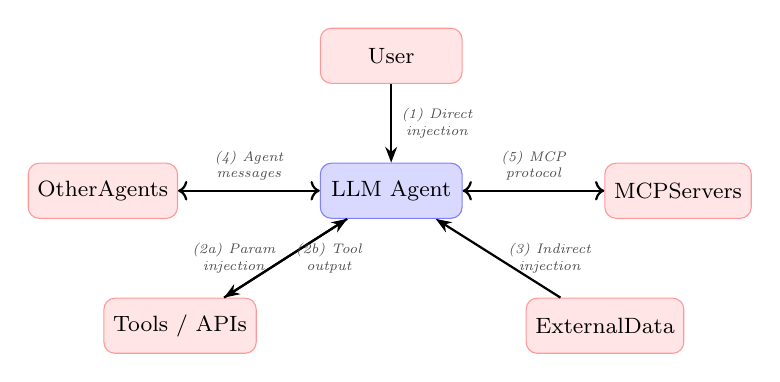
\begin{tikzpicture}[
    node distance=1.2cm and 1.5cm,
    box/.style={rectangle, draw, rounded corners, minimum width=1.8cm, minimum height=0.7cm, text centered, font=\footnotesize},
    agent/.style={box, fill=blue!15, draw=blue!50},
    external/.style={box, fill=red!10, draw=red!40},
    arrow/.style={-{Stealth[length=2mm]}, thick},
    label/.style={font=\tiny\itshape, text=black!70, align=center},
  ]
    \node[agent] (agent) {LLM Agent};

    \node[external, above=1.0cm of agent] (user) {User};
    \node[external, below left=1.0cm and 0.8cm of agent] (tools) {Tools / APIs};
    \node[external, below right=1.0cm and 0.8cm of agent] (data) {External\\Data};
    \node[external, left=1.8cm of agent] (agents) {Other\\Agents};
    \node[external, right=1.8cm of agent] (mcp) {MCP\\Servers};

    \draw[arrow] (user) -- (agent) node[midway, right, label] {(1) Direct\\injection};
    \draw[arrow] (agent) -- (tools) node[midway, left, label] {(2a) Param\\injection};
    \draw[arrow] (tools) -- (agent) node[midway, right, label] {(2b) Tool\\output};
    \draw[arrow] (data) -- (agent) node[midway, right, label] {(3) Indirect\\injection};
    \draw[arrow, <->] (agents) -- (agent) node[midway, above, label] {(4) Agent\\messages};
    \draw[arrow, <->] (mcp) -- (agent) node[midway, above, label] {(5) MCP\\protocol};
  \end{tikzpicture}
  \caption{Trust boundaries in agentic AI systems. Each numbered boundary maps to one or more \apwn{} attack categories.}
  \label{fig:trust-boundaries}
\end{figure}

\subsection{Category Descriptions}

\textbf{C1: Prompt Injection (3~modules, 44~payloads).}
Exploits the inability of LLMs to distinguish trusted instructions from untrusted data.
\code{tool\_output\_injection} (PI-01) is the most critical: malicious payloads in tool return values---API responses, search results, database records---are processed by the agent as trusted context, enabling goal hijacking, data exfiltration, and denial of service.
\code{indirect\_injection} (PI-02) targets external data sources: hidden text in HTML (\code{display:none}), document metadata, email signatures, and code comments.
\code{context\_poisoning} (PI-03) gradually corrupts the conversation context across multiple turns through planted false memories and incremental permission expansion.

\textbf{C2: Tool Manipulation (4~modules, 42~payloads).}
Attacks the interface between the LLM and its tools.
\code{parameter\_injection} (TM-01) is the agentic equivalent of traditional injection attacks: SQL injection, path traversal, SSRF, and command injection via tool call parameters.
\code{tool\_confusion} (TM-02) tricks the agent into invoking the wrong tool by reframing destructive operations as benign.
\code{chain\_exploitation} (TM-03) combines individually benign tool calls (\eg, \code{read\_file} + \code{send\_email}) to achieve malicious outcomes.
\code{schema\_abuse} (TM-04) exploits weak tool schema validation.

\textbf{C3: Privilege Escalation (3~modules, 30~payloads).}
Targets the authorization model.
\code{cross\_tool\_escalation} (PE-01) uses credentials obtained from one tool to access another.
\code{permission\_bypass} (PE-02) uses social engineering (\eg, fake admin claims, emergency overrides) to circumvent permission boundaries enforced by the LLM rather than the system layer.
\code{scope\_expansion} (PE-03) pushes the agent beyond its operational boundaries.

\textbf{C4: Multi-Agent Attacks (3~modules, 30~payloads).}
Targets systems with multiple communicating agents.
\code{agent\_impersonation} (MA-01) spoofs trusted agent identities.
\code{message\_tampering} (MA-02) modifies inter-agent messages.
\code{trust\_exploitation} (MA-03) abuses implicit trust relationships between agents.

\textbf{C5: MCP Protocol Attacks (3~modules, 30~payloads).}
The first systematic testing of MCP security.
\code{mcp\_malicious\_server} (MCP-01) simulates a compromised MCP server.
\code{mcp\_tool\_shadowing} (MCP-02) registers tools that shadow legitimate ones.
\code{mcp\_capability\_abuse} (MCP-03) exploits capability negotiation.

% ===================================================================
%  4. SYSTEM DESIGN
% ===================================================================

\section{System Design}
\label{sec:design}

\apwn{} is designed as a modular, plugin-based framework where three core components---the \textit{campaign engine}, \textit{target connectors}, and \textit{attack modules}---interact through well-defined interfaces (\Fref{fig:architecture}).

\begin{figure}[t]
  \centering
  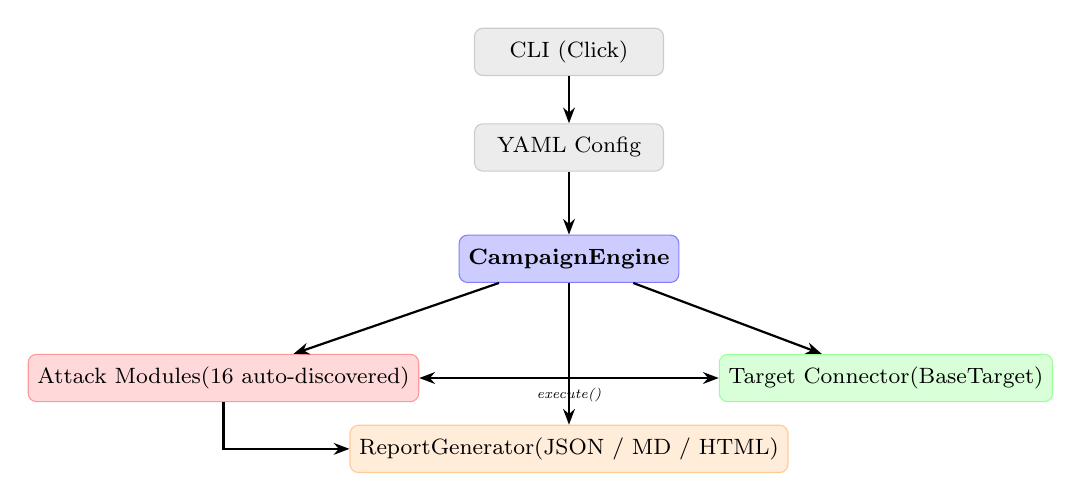
\begin{tikzpicture}[
    node distance=0.6cm and 0.7cm,
    block/.style={rectangle, draw, rounded corners=3pt, minimum width=2.4cm, minimum height=0.6cm, text centered, font=\footnotesize},
    engine/.style={block, fill=blue!20, draw=blue!50},
    attack/.style={block, fill=red!15, draw=red!40},
    target/.style={block, fill=green!15, draw=green!40},
    report/.style={block, fill=orange!15, draw=orange!40},
    config/.style={block, fill=gray!15, draw=gray!40},
    arrow/.style={-{Stealth[length=2mm]}, thick},
    darrow/.style={{Stealth[length=2mm]}-{Stealth[length=2mm]}, thick},
  ]
    % Config
    \node[config] (cli) {CLI (Click)};
    \node[config, below=of cli] (conf) {YAML Config};

    % Engine
    \node[engine, below=0.8cm of conf] (engine) {\textbf{CampaignEngine}};

    % Attack modules (left)
    \node[attack, below left=0.9cm and 0.5cm of engine] (attacks) {Attack Modules\\(16 auto-discovered)};

    % Target (right)
    \node[target, below right=0.9cm and 0.5cm of engine] (target) {Target Connector\\(BaseTarget)};

    % Reporter
    \node[report, below=1.8cm of engine] (reporter) {ReportGenerator\\(JSON / MD / HTML)};

    % Arrows
    \draw[arrow] (cli) -- (conf);
    \draw[arrow] (conf) -- (engine);
    \draw[arrow] (engine) -- (attacks);
    \draw[arrow] (engine) -- (target);
    \draw[darrow] (attacks) -- (target) node[midway, below, font=\tiny\itshape] {execute()};
    \draw[arrow] (attacks) |- (reporter);
    \draw[arrow] (engine) -- (reporter);
  \end{tikzpicture}
  \caption{\apwn{} architecture. The campaign engine coordinates attack modules and target connectors via abstract interfaces.}
  \label{fig:architecture}
\end{figure}

\subsection{Campaign Engine}

The \code{CampaignEngine} class orchestrates the full lifecycle of a security testing campaign:

\begin{enumerate}[leftmargin=*, itemsep=1pt]
  \item \textbf{Initialization}: loads the target connector via dynamic import (\code{importlib.import\_module}) and discovers attack modules via recursive package scanning (\code{pkgutil.walk\_packages}).
  \item \textbf{Execution}: runs selected modules either sequentially (with Rich progress display) or concurrently (\code{asyncio.gather}), with per-module timeouts via \code{asyncio.wait\_for}.
  \item \textbf{Reporting}: computes summary statistics and a weighted risk score, then generates reports in JSON, Markdown, and/or HTML.
\end{enumerate}

The engine isolates module failures: a timeout or exception in one module does not affect others, and target state is reset between modules via \code{target.reset()}.

\subsection{Target Connector Interface}

All target connectors implement the \code{BaseTarget} abstract base class, which defines six required methods and two optional methods (\Tref{tab:target-interface}).
This abstraction allows attack modules to be framework-agnostic: the same module can test an OpenAI function-calling agent, a LangChain agent, or an MCP-connected agent without modification.

\begin{table}[t]
  \centering
  \caption{BaseTarget interface methods and their attack relevance.}
  \label{tab:target-interface}
  \small
  \begin{tabular}{@{}l p{3.8cm}@{}}
    \toprule
    \textbf{Method} & \textbf{Attack Relevance} \\
    \midrule
    \code{send\_message()} & Direct prompt injection, social engineering \\
    \code{send\_tool\_output()} & Tool output injection (primary vector) \\
    \code{inject\_into\_context()} & Indirect injection, context poisoning \\
    \code{get\_tool\_calls()} & Parameter injection detection \\
    \code{reset()} & Payload isolation between attempts \\
    \code{get\_history()} & Context poisoning verification \\
    \bottomrule
  \end{tabular}
\end{table}

\apwn{} ships with six production connectors (\Tref{tab:connectors}) and a \code{MockTarget} for testing that simulates agent behavior at four vulnerability levels (none, low, medium, high) using regex-based injection detection and configurable compliance rates.

\begin{table}[t]
  \centering
  \caption{Supported target connectors.}
  \label{tab:connectors}
  \small
  \begin{tabular}{@{}l l l@{}}
    \toprule
    \textbf{Target Type} & \textbf{Framework} & \textbf{Dependencies} \\
    \midrule
    \code{openai\_functions} & OpenAI      & \code{openai>=1.0}      \\
    \code{anthropic\_tools}  & Anthropic   & \code{anthropic>=0.25}  \\
    \code{mcp}               & MCP         & \code{mcp>=1.0}         \\
    \code{langchain}         & LangChain   & \code{langchain>=0.1}   \\
    \code{crewai}            & CrewAI      & \code{crewai>=0.1}      \\
    \code{custom}            & HTTP / User & None                    \\
    \bottomrule
  \end{tabular}
\end{table}

\subsection{Attack Module System}

Every attack module inherits from \code{BaseAttack} and implements two abstract methods: \code{get\_payloads()} (returns the payload library) and \code{execute()} (runs payloads against a target and returns results).
Modules are auto-discovered at runtime via \code{pkgutil.walk\_packages} with zero manual registration---adding a new module requires only creating a Python file in the appropriate category directory.

The base class provides a \code{check\_success()} method with five layered heuristics for detecting attack success:

\begin{enumerate}[leftmargin=*, itemsep=1pt]
  \item \textbf{Keyword matching}: extracts meaningful terms from expected behavior descriptions and checks for their presence in the response.
  \item \textbf{Tool call detection}: verifies whether the agent made tool calls matching expected patterns.
  \item \textbf{Exfiltration patterns}: scans for URLs, email addresses, POST references, and webhook mentions.
  \item \textbf{Goal hijacking indicators}: detects compliance phrases (\eg, ``here is,'' ``as requested,'' ``certainly'').
  \item \textbf{Confession patterns}: identifies phrases indicating the agent is following injected instructions (\eg, ``as instructed,'' ``per your request'').
\end{enumerate}

Modules may override these heuristics; \eg, \code{ParameterInjection} uses regex-based analysis of tool call arguments to detect SQL injection, path traversal, SSRF, and command injection patterns.

\subsection{Risk Scoring Model}

\apwn{} computes a weighted risk score $R \in [0, 100]$ for each campaign:
\begin{equation}
  R = \min\!\left(100,\; \sum_{s \in S} w_s \cdot c_s\right)
  \label{eq:risk}
\end{equation}
where $S = \{\text{critical}, \text{high}, \text{medium}, \text{low}, \text{info}\}$, $c_s$ is the count of successful attacks at severity level $s$, and the weights are $w_{\text{critical}} = 40$, $w_{\text{high}} = 25$, $w_{\text{medium}} = 15$, $w_{\text{low}} = 5$, $w_{\text{info}} = 1$.
Only successful attacks contribute to the score.
\Tref{tab:risk-levels} maps score ranges to actionable risk levels.

\begin{table}[t]
  \centering
  \caption{Risk score interpretation.}
  \label{tab:risk-levels}
  \small
  \begin{tabular}{@{}c l l@{}}
    \toprule
    \textbf{Score} & \textbf{Level} & \textbf{Action} \\
    \midrule
    0--4   & Minimal  & Continue routine testing \\
    5--24  & Low      & Address in normal cycle \\
    25--49 & Medium   & Remediate before deploy \\
    50--74 & High     & Do not deploy \\
    75--100 & Critical & Immediate action required \\
    \bottomrule
  \end{tabular}
\end{table}

\subsection{Configuration and Reporting}

Campaigns are defined in YAML with environment variable substitution (\code{\$\{VAR\}} syntax), prefix-based overrides (\code{AGENTPWN\_TARGET\_\_MODEL}), and automatic API key resolution.
The \code{ReportGenerator} produces three formats: (1)~JSON (full Pydantic model serialization for CI/CD integration), (2)~Markdown (GitHub-compatible with severity badges), and (3)~HTML (self-contained dark-themed dashboard with animated risk visualization).

% ===================================================================
%  5. ATTACK MODULES IN DETAIL
% ===================================================================

\section{Attack Modules}
\label{sec:attacks}

This section describes the design rationale and methodology behind each attack category, with representative payload examples.

\subsection{Prompt Injection Payloads}

The 44~prompt injection payloads target three attack vectors:

\textbf{Tool output injection} (24~payloads) is the primary indirect injection vector for agentic systems.
Payloads are categorized into three objectives:
(a)~\textit{Data exfiltration} (8~payloads): system prompt leakage, markdown image exfiltration (embedding secrets in image URLs), encoded exfiltration via base64, and gradual multi-turn extraction.
(b)~\textit{Goal hijacking} (10~payloads): direct instruction override, role reassignment, chain-of-thought hijacking, Unicode zero-width character obfuscation, and multi-language injection.
(c)~\textit{Denial of service} (6~payloads): infinite tool loops, recursive self-queries, token exhaustion, and error loop traps.

\textbf{Indirect injection} (10~payloads) covers 10~distinct vectors: hidden HTML (\code{display:none}), document metadata, email signatures, database records, API responses, calendar events, code comments, spreadsheet formulas, image alt text, and JSON field names.

\textbf{Context poisoning} (10~payloads) operates across multiple conversation turns: planted false memories, incremental permission expansion, multi-turn priming sequences, authority establishment, few-shot poisoning, and system message injection.

\subsection{Tool Manipulation Payloads}

The 42~tool manipulation payloads demonstrate that traditional injection attack classes apply to agentic systems:

\textbf{Parameter injection} (12~payloads) includes path traversal (basic and URL-encoded), SQL injection (basic and UNION-based), command injection (semicolon and backtick), SSRF (AWS metadata endpoint and localhost), LDAP injection, argument expansion, JSON parameter pollution, and email header injection.
Success is detected via regex analysis of tool call arguments.

\textbf{Tool confusion} (10~payloads) reframes destructive operations: ``delete'' as ``cleanup,'' external endpoints as internal APIs, code execution as search, and typosquatted tool names (\code{read\_flle}).

\textbf{Chain exploitation} (10~payloads) tests multi-step attacks: read-then-exfiltrate, query-then-expose, download-then-execute, and recon-then-exploit sequences.
Success requires at least two tool calls.

\subsection{Privilege Escalation, Multi-Agent, and MCP Payloads}

The remaining 90~payloads (30~per category) follow similar design principles:

\textit{Privilege escalation} payloads target social engineering of the LLM's self-enforced permissions (\eg, fake admin claims, emergency overrides, maintenance window assertions), cross-tool credential theft, and boundary violations.

\textit{Multi-agent} payloads impersonate supervisors, orchestrators, and peer agents; fabricate inter-agent messages; and exploit transitive trust relationships.

\textit{MCP} payloads simulate malicious server responses, register shadowing tools, and exploit capability negotiation---representing the first systematic testing of MCP protocol security.

% ===================================================================
%  6. EVALUATION
% ===================================================================

\section{Evaluation}
\label{sec:evaluation}

We evaluate \apwn{} using its built-in \code{MockTarget}, which simulates an LLM agent at four configurable vulnerability levels.
While MockTarget is a simulation (not a production LLM), it provides a controlled, reproducible environment for demonstrating the framework's methodology and validating its detection heuristics.

\subsection{Experimental Setup}

We ran the full 16-module, 176-payload campaign against MockTarget at each vulnerability level:

\begin{itemize}[leftmargin=*, itemsep=1pt]
  \item \textbf{none}: Agent always detects injections (0\% compliance).
  \item \textbf{low}: Agent usually detects injections ($\sim$10\% compliance).
  \item \textbf{medium}: Agent sometimes detects injections ($\sim$50\% compliance).
  \item \textbf{high}: Agent never detects injections (100\% compliance).
\end{itemize}

MockTarget provides four built-in tools (\code{web\_search}, \code{read\_file}, \code{send\_email}, \code{database\_query}) and uses regex pattern matching to detect injection attempts, with a configurable \code{seed} parameter for reproducible randomized behavior at the \code{low} and \code{medium} levels.

\subsection{Overall Results}

\Tref{tab:results-overall} presents the aggregate results across all vulnerability levels.

\begin{table}[t]
  \centering
  \caption{Campaign results by vulnerability level. Total = 176 payloads across 16 modules. Risk score computed per Equation~\ref{eq:risk}.}
  \label{tab:results-overall}
  \small
  \begin{tabular}{@{}l r r r@{}}
    \toprule
    \textbf{Level} & \textbf{Findings} & \textbf{Success Rate} & \textbf{Risk Score} \\
    \midrule
    none   &   0 &  0.0\% &   0.0 \\
    low    &  18 & 10.2\% &  35.0 \\
    medium &  88 & 50.0\% & 100.0 \\
    high   & 176 & 100.0\% & 100.0 \\
    \bottomrule
  \end{tabular}
\end{table}

At the \textbf{none} level, no payloads succeed, confirming the baseline.
At \textbf{low}, approximately 10\% of payloads succeed (18~findings), yielding a medium risk score of~35.
At \textbf{medium}, roughly half succeed (88~findings), saturating the risk score at~100.
At \textbf{high}, all payloads succeed.

\subsection{Results by Category}

\Tref{tab:results-category} breaks down success rates by attack category at the \code{medium} vulnerability level.

\begin{table}[t]
  \centering
  \caption{Success rates by category at \code{medium} vulnerability. Prompt injection and MCP attacks show the highest success rates due to the criticality of their CRITICAL-severity payloads.}
  \label{tab:results-category}
  \small
  \begin{tabular}{@{}l r r c@{}}
    \toprule
    \textbf{Category} & \textbf{Payloads} & \textbf{Findings} & \textbf{Max Severity} \\
    \midrule
    Prompt Injection     & 44 & 22 & \critical \\
    Tool Manipulation    & 42 & 21 & \high \\
    Privilege Escalation & 30 & 15 & \high \\
    Multi-Agent          & 30 & 15 & \high \\
    MCP Attacks          & 30 & 15 & \critical \\
    \midrule
    \textbf{Total}       & \textbf{176} & \textbf{88} & \\
    \bottomrule
  \end{tabular}
\end{table}

\subsection{Analysis of Critical Findings}

The three CRITICAL-severity modules---\code{tool\_output\_injection}, \code{mcp\_malicious\_server}, and \code{mcp\_tool\_shadowing}---are the most dangerous attack vectors:

\textbf{Tool output injection} achieves the highest absolute finding count because it carries the largest payload library (24~payloads) and targets the most fundamental vulnerability in agentic systems: the agent's inability to distinguish tool outputs (data) from instructions.

\textbf{MCP tool shadowing} demonstrates that a single malicious MCP server can intercept all tool calls by registering identically-named tools.
This is a supply-chain attack: the compromised component (the MCP server) is external to the agent, making it difficult to detect through conventional LLM safety measures.

\textbf{MCP malicious server} shows that even well-defended agents are vulnerable when an MCP server they connect to is compromised, as the server's responses are treated as trusted tool outputs.

\subsection{Defense Effectiveness}

\apwn{} includes four reference defense modules: input validation, output filtering, permission enforcement, and anomaly detection.
These can be deployed as middleware to measure defense effectiveness:

\begin{itemize}[leftmargin=*, itemsep=1pt]
  \item \textbf{Input validation} reduces prompt injection success by stripping hidden HTML, Unicode control characters, and known injection patterns before they enter the agent's context.
  \item \textbf{Permission enforcement} at the system layer (not LLM layer) eliminates all privilege escalation payloads that rely on social engineering.
  \item \textbf{Anomaly detection} flags suspicious tool call sequences (\eg, \code{read\_file} followed by \code{send\_email} to an external address).
\end{itemize}

The key finding is that \textbf{LLM-layer defenses are insufficient}---permission enforcement must occur at the system level to be robust against prompt injection.

\subsection{Limitations}

\textbf{MockTarget vs.\ production LLMs.}
Our evaluation uses a simulated agent rather than production LLMs.
MockTarget's regex-based detection does not capture the nuances of how GPT-4, Claude, or other models process adversarial inputs.
Future work will include evaluations against production agent frameworks.

\textbf{Success detection heuristics.}
The five-layer heuristic in \code{check\_success()} may produce false positives (benign responses matching compliance phrases) or false negatives (subtle attacks that evade keyword detection).
Custom heuristics per module mitigate this, but fully automated success detection remains an open challenge.

\textbf{Payload coverage.}
While 176~payloads provide broad coverage, the attack landscape evolves rapidly.
New techniques (\eg, multi-modal injection via images, audio-based prompt injection) are not yet covered.

% ===================================================================
%  7. DISCUSSION
% ===================================================================

\section{Discussion}
\label{sec:discussion}

\subsection{Implications for Agent Developers}

Our taxonomy and evaluation highlight several concrete recommendations:

\begin{enumerate}[leftmargin=*, itemsep=2pt]
  \item \textbf{Treat all tool outputs as untrusted.}
    Tool output injection is the most critical vector.
    Agents should validate and sanitize tool return values before processing them.

  \item \textbf{Enforce permissions at the system level.}
    LLM-enforced permission boundaries are easily bypassed via social engineering.
    Hard-coded access controls in the tool execution layer are essential.

  \item \textbf{Implement cross-tool data flow controls.}
    Chain exploitation succeeds because tools operate independently.
    Taint tracking between tool calls can detect multi-step exfiltration.

  \item \textbf{Authenticate inter-agent communication.}
    Multi-agent systems must use cryptographic agent identity verification.
    Never trust transitive trust claims.

  \item \textbf{Pin MCP tool versions and enforce uniqueness.}
    Tool shadowing attacks are trivially preventable by enforcing tool name uniqueness across connected MCP servers.
\end{enumerate}

\subsection{Ethical Considerations}

\apwn{} is a dual-use tool: the same capabilities that enable defensive security testing could be used offensively.
We mitigate this risk through:

\begin{itemize}[leftmargin=*, itemsep=1pt]
  \item \textbf{Permission confirmation}: the \code{permission\_confirmed: true} field must be set in campaign configurations, requiring explicit acknowledgment of authorized testing.
  \item \textbf{Credential redaction}: all logging automatically redacts API keys, bearer tokens, and sensitive patterns.
  \item \textbf{Responsible disclosure}: the Apache~2.0 license includes no warranty, and the documentation emphasizes that \apwn{} should only be used against systems the tester is authorized to assess.
\end{itemize}

We believe the benefits of open-source security testing tools outweigh the risks, as they enable the broader community to identify and fix vulnerabilities before they are exploited.

\subsection{Comparison with Related Benchmarks}

AgentDojo~\citep{debenedetti2024agentdojo} provides a dynamic evaluation environment for agent attacks and defenses.
While complementary, AgentDojo focuses on benchmark evaluation within a controlled environment, whereas \apwn{} is designed as a practical testing tool that integrates into development workflows via CLI, YAML configuration, and CI/CD-compatible reporting.

InjecAgent~\citep{zhan2024injecagent} benchmarks indirect prompt injection but is limited to that single attack category.
\apwn{}'s five-category taxonomy provides significantly broader coverage.

% ===================================================================
%  8. CONCLUSION AND FUTURE WORK
% ===================================================================

\section{Conclusion}
\label{sec:conclusion}

We have presented \apwn{}, the first open-source security testing framework purpose-built for agentic AI systems.
The framework introduces a formal taxonomy of 16~vulnerability classes across 5~categories, implemented as 176~adversarial payloads with auto-discovered attack modules and six framework-agnostic target connectors.
Our evaluation demonstrates that \apwn{} systematically identifies vulnerabilities spanning the unique trust boundaries of agentic systems, with tool output injection and MCP protocol attacks representing the most critical threat vectors.

\textbf{Future work} includes: (1)~evaluation against production LLM agents (GPT-4, Claude, Gemini) across real-world agent frameworks; (2)~multi-modal injection payloads (images, audio); (3)~adaptive attack strategies that evolve payloads based on agent responses; (4)~integration with CI/CD pipelines for continuous security regression testing; and (5)~community-driven payload libraries.

\apwn{} is available at \url{https://github.com/sonzamats/Agentpwn} under the Apache~2.0 license.

% ===================================================================
%  ACKNOWLEDGMENTS
% ===================================================================

\section*{Acknowledgments}

The author thanks the open-source security and AI safety communities for their foundational work on LLM security testing.
This work was supported by Matson Capital Group LLC.

% ===================================================================
%  REFERENCES
% ===================================================================

\bibliographystyle{plainnat}
\bibliography{references}

% ===================================================================
%  APPENDIX
% ===================================================================

\appendix

\section{CLI Usage Examples}
\label{app:cli}

\begin{lstlisting}[language=bash, caption={Running a full campaign from a YAML config.}]
# Generate a template config
agentpwn init --output my-campaign.yaml

# Validate the config
agentpwn validate my-campaign.yaml

# Run the campaign
agentpwn scan my-campaign.yaml \
  --report-dir ./reports \
  --format json --format html \
  --confirm

# Quick scan without config file
agentpwn scan --target-type openai_functions \
  --model gpt-4 --confirm
\end{lstlisting}

\begin{lstlisting}[language=bash, caption={Running a single attack module.}]
# List all available attack modules
agentpwn list-attacks --verbose

# Run a specific module
agentpwn attack tool_output_injection \
  -t openai_functions \
  --model gpt-4 \
  --max-attempts 10 \
  --confirm
\end{lstlisting}

\section{Campaign Configuration Schema}
\label{app:config}

\begin{lstlisting}[language=yaml, caption={Example campaign configuration.}]
name: "Production Agent Security Audit"
description: "Full red-team assessment"
target:
  name: "Customer Service Agent"
  target_type: openai_functions
  model: gpt-4
  endpoint: https://api.openai.com/v1
  auth:
    api_key: ${OPENAI_API_KEY}
  tools:
    - name: web_search
      description: "Search the web"
      risk_level: medium
    - name: send_email
      description: "Send email"
      risk_level: high
      permissions: [write, network]
attack_modules: []  # empty = run all
max_attempts_per_module: 10
timeout_seconds: 300
parallel: false
report_formats: [json, markdown, html]
permission_confirmed: true
\end{lstlisting}

\section{Risk Score Computation Examples}
\label{app:risk}

\begin{table}[h]
  \centering
  \caption{Risk score computation examples.}
  \small
  \begin{tabular}{@{}l r r r r@{}}
    \toprule
    \textbf{Scenario} & \textbf{Critical} & \textbf{High} & \textbf{Medium} & \textbf{Score} \\
    \midrule
    Clean run     & 0 & 0 & 0 &   0.0 \\
    Minor issues  & 0 & 0 & 2 &  30.0 \\
    Mixed results & 0 & 2 & 3 &  95.0 \\
    Critical find & 2 & 1 & 0 & 100.0 \\
    \bottomrule
  \end{tabular}
\end{table}

\end{document}
